\documentclass[5pt]{article}
\usepackage{multicol,multirow}
\usepackage{graphicx} % Required for inserting images
\usepackage[margin=0.75cm]{geometry}
\usepackage{xcolor}
\usepackage{amsmath}
\usepackage{mathtools}
\usepackage{relsize}


\usepackage{empheq}
\usepackage{amsfonts}

\usepackage{tkz-euclide}
\usepackage{tikz}

\definecolor{LightGray}{gray}{0.9}

\usepackage{minted}

\DeclarePairedDelimiter\abs{\lvert}{\rvert}%
\DeclarePairedDelimiter\norm{\lVert}{\rVert}%

\makeatletter
\let\oldabs\abs
\def\abs{\@ifstar{\oldabs}{\oldabs*}}

\newcommand{\tr}[3]{
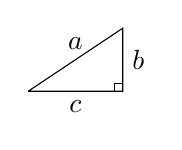
\begin{tikzpicture}[scale=0.40]
    \coordinate [] (A) at (-1.5cm,-1.cm);
    \coordinate [] (C) at (1.5cm,-1.0cm);
    \coordinate [] (B) at (1.5cm,1.0cm);
    \draw (A) -- node[above] {$a$} (B) -- node[right] {$b$} (C) -- node[below] {$c$} (A);
    \draw (1.25cm,-1.0cm) rectangle (1.5cm,-0.75cm);
\end{tikzpicture}
}


\begin{document}


\begin{center}
     \Large{\textbf{Calculus 2 For Engineers}}\\
     \small{Class: APPM 1360}\hfill\small{\textcopyright Maximilien Notz \the\year{}}
     \noindent\rule{20.2cm}{0.4pt}
\end{center}


\begin{multicols}{2}
\setcounter{secnumdepth}{0}


\section{Trig. Formula}
\subsection{Integral's}
$\int \sec{x}\,dx=ln|\sec{x}+\tan{x}|+c$\\
$\int \csc{x}\,dx=ln|\csc{x}+\cot{x}|+c$\\
\subsection{Identity's}
\begin{tabular}{l|l}
$\sin^2{x}+\cos^2{x} = 1$ & $\sin^2{x}=\frac{1}{2}(1-\cos{2x})$\\
$\sin{2x} = 2\sin{x}\cos{x}$ & $\sec^2{x}=1+\tan^2{x}$\\
$\cos^2{x}=\frac{1}{2}(1+\cos{2x})$ & \\
\end{tabular}




\section{Integration technique}
\begin{tabular}{ll}
    Integration by part & $\int udv=uv-\int vdu$\\
    Trig. Integration method & $\int f^3(x)dx=\int f^2(x)f(xt)dx$\\
    Trig. Substitution:   & \\
\end{tabular}
    
\begin{tabular}{c|c|c|c}
    Integrand & Substitution & Bound & Triangle\\
    \hline
    $\sqrt{a^2-x^2}$ & $x=a\sin{\theta}$ & $-\frac{\pi}{2}\le\theta\le\frac{\pi}{2}$ & fig. 1\\
    $\sqrt{a^2+x^2}$ & $x=a\tan{\theta}$ & $-\frac{\pi}{2}\le\theta\le\frac{\pi}{2}$ & fig. 2\\
    $\sqrt{x^2-a^2}$ & $x=a\sec{\theta}$ & ... & fig. 3\\
\end{tabular}

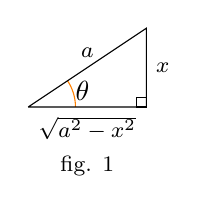
\begin{tikzpicture}[scale=0.50]
\coordinate [] (A) at (-1.5cm,-1.cm);
\coordinate [] (C) at (1.5cm,-1.0cm);
\coordinate [] (B) at (1.5cm,1.0cm)pic["$\theta$", draw=orange, -, angle eccentricity=1.2, angle radius=0.6cm]{angle=C--A--B};
\draw (A) -- node[above] {\footnotesize{$a$}} (B) -- node[right] {\footnotesize{$x$}} (C) -- node[below] {\footnotesize{$\sqrt{a^2-x^2}$}} (A);
\draw (1.25cm,-1.0cm) rectangle (1.5cm,-0.75cm);
\node[anchor = south] at (0,-3){\footnotesize fig. 1};
\end{tikzpicture}
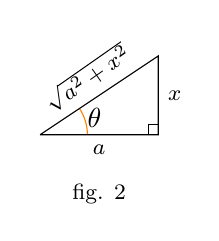
\begin{tikzpicture}[scale=0.50]
\coordinate [] (A) at (-1.5cm,-1.cm);
\coordinate [] (C) at (1.5cm,-1.0cm);
\coordinate [] (B) at (1.5cm,1.0cm)pic["$\theta$", draw=orange, -, angle eccentricity=1.2, angle radius=0.6cm]{angle=C--A--B};
\draw (A) -- node[above, rotate=35] {\footnotesize{$\sqrt{a^2+x^2}$}} (B) -- node[right] {\footnotesize{$x$}} (C) -- node[below] {\footnotesize{$a$}} (A);
\draw (1.25cm,-1.0cm) rectangle (1.5cm,-0.75cm);
\node[anchor = south] at (0,-3){\footnotesize fig. 2};
\end{tikzpicture}
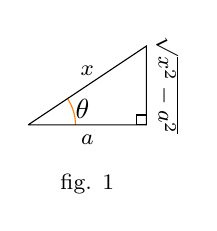
\begin{tikzpicture}[scale=0.50]
\coordinate [] (A) at (-1.5cm,-1.cm);
\coordinate [] (C) at (1.5cm,-1.0cm);
\coordinate [] (B) at (1.5cm,1.0cm)pic["$\theta$", draw=orange, -, angle eccentricity=1.2, angle radius=0.6cm]{angle=C--A--B};
\draw (A) -- node[above] {\footnotesize{$x$}} (B) -- node[right, anchor = south, rotate=270] {\footnotesize{$\sqrt{x^2-a^2}$}} (C) -- node[below] {\footnotesize{$a$}} (A);
\draw (1.25cm,-1.0cm) rectangle (1.5cm,-0.75cm);
\node[anchor = south] at (0,-3){\footnotesize fig. 1};
\end{tikzpicture}



\section{Partial Fraction}
$\dfrac{N(x)}{(ax+b)^2}=\dfrac{A}{ax+b}+\dfrac{B}{(ax+b)^2}$\\
$\dfrac{N(x)}{(ax+b)(cx+d)}=\dfrac{A}{ax+b}+\dfrac{B}{cx+d}$\\
$\dfrac{N(x)}{(ax+b)(cx+d)^2}=\dfrac{A}{ax+b}+\dfrac{B}{(cx+d)^2}$\\


\section{Integral Approximation}
\subsection{Riemann Sum Rules}
\begin{tabular}{ll }
    Delta X & $\Delta x=\dfrac{b-a}{n}$\\
    Right Endpoint & $R_n=\mathlarger{\sum_{i=1}^n}\Delta xf(x_i)$\\
     & $x_i=a+i\Delta x$\\
    Left Endpoint & $L_n=\mathlarger{\sum_{i=0}^{n-1 }}\Delta xf(x_i)$\\
     & $x_i=a+i\Delta x$\\
    Midpoint & $M_n=\mathlarger{\sum_{i=0}^n}\Delta xf(\overline{x}_i)$\\
     & $\overline{x}_i=\dfrac{x_{i-1}+x_i}{2}$\\
    Trapezoidal & $T_n=\frac{\Delta x}{2}(f(a)+2f(x_1)+...+2f(x_{n-1})+f(b))$
\end{tabular}
\subsection{Short Formula}
$L_n=[f(a)+f(a+\Delta x)+f(a+2\Delta x)+...++f(b-\Delta x)]$\\
$R_n=[f(a+\Delta x)+f(a+\Delta x)+f(a+2\Delta x)+...++f(b)]$\\
$M_n=[f(a+\frac{\Delta x}{2})+f(a+\frac{3\Delta x}{2})+...+f(b-\frac{\Delta x}{2})]$\\
$T_n=\dfrac{\Delta x}{2}[f(a)+2f(a+\Delta x)+2f(a+2\Delta x)+...+f(b)]$

\section{Error}
\subsection{Exact Error}
\begin{tabular}{ll}
     Trapezoidal Exact Er. & $E_T=T_N-\int_a^bf(x)dx$\\
     Midpoint Exact Er. & $E_M=T_M-\int_a^bf(x)dx$\\
\end{tabular}

\subsection{Bound Error}
Suppose that $|f''(x)|\le K$ for $a\le x\le a$ and let $N$ be the amount of iteration.\\
\begin{tabular}{ll}
Trapezoidal Er. & $E_T\le\dfrac{K(b-a)^3}{12N^2}$\\
Midpoint Er. & $E_M\le\dfrac{K(b-a)^3}{24N^2}$\\
\end{tabular}
\section{Comparison Thm}
Supose that $f(x)$ and $g(x)$ are continuous function with $f(x)\geq g(x)\geq0$ for $x\geq a$.\\
1. If $\int^\infty_af(x)dx$ is  convergent, then $\int^\infty_ag(x)dx$ is convergent.\\
2. If $\int^\infty_ag(x)dx$ is  divergent, then $\int^\infty_ag(x)dx$ is divergent.\\
\\
p-series $\int^\infty_1\frac{1}{x^p}dx$ is convergent if $p>1$ and divergent if $p\le 1$.\\

\section{Volumes}
\begin{tabular}{ll}
    General Formula & $V=\int_a^bA(x)\,dx$\\
    Disc. Method & $V=\int_a^b\pi R^2(x)\,dx$\\
    Washer Method & $V=\int_a^b\pi R^2-\pi r^2$\\
    Cylindrical Shell & $V=\int_a^b2\pi R(x)h(x)\,dx$\\
\end{tabular}
\section{Surface area}
\begin{tabular}{ll}
    Arc-length & $L=\int_a^bds=\int_a^b\sqrt{1+[f'(x)]^2}\, dx$ \\
    Surface    & $SA=\int_a^bdA=\int_a^b2\pi r ds$\\
               & $=\int_a^b2\pi r \sqrt{1+(y')^2}dx$\\
\end{tabular}
\section{Center of mass}
\begin{tabular}{ll}
    $(\overline{x}, \overline{y})$ & $\overline{x}=\frac{M_y}{M}=\frac{\sum^n_{i=1}m_i\,x_i}{M},\;\overline{y}=\frac{M_x}{M}=\frac{\sum^n_{i=1}m_i\,y_i}{M}$ \\
    density & $\rho=\frac{m}{A}$\\
    & $m=\rho\int^b_a[f(x)-g(x)]dx$
    
\end{tabular}


\section{Differential Equation}
\subsubsection{Separable Equation}
\begin{enumerate}
    \item $\frac{dy}{dx}=g(x)f(y)$
    \item $\int f(y)dy=\int \frac{1}{g(x)}dx$
\end{enumerate}


\section{Sequence \& Series}
\subsection{Sequence}
\begin{tabular}{ll}
    Factoriel     & $n!=1\cdot2\cdot3\cdot ...\cdot n$\\
                  & $n!=n(n-1)(n-2)...2\cdot1$\\
                  & $0!=1$\\
    Geometric     & $\{r^N\}^\infty_{n=0}=\{1,r^1,r^2,...\}$\\
    Increasing    & If $a_n< a_{n+1}$\\
    Convergence   & \(\lim\limits_{x\to\infty} a_n\) exist and is $\infty$ then we say the\\
                  & sequence \textbf{converges} and \textbf{diverges} otherwise.\\
    Limit         & \(\lim\limits_{x\to\infty} a_n=L\)\\
    Monotonic     & If it is \textbf{increasing} or \textbf{decreasing}.\\
    Bounded       & If it  is bounded \textbf{above} or \textbf{below}.\\
    Bounded above & If there is a number $m$ such that\\
                  & $a_n\leq m, \forall n\geq1$\\
    Recursive  & \underline{Ex:} Let $a_1=1, a_n=2a_{N-1}+1$\\
\end{tabular}

\subsection{Series convergence tests}

\subsubsection{Geometric serie}
for $\sum a_n=\sum A r^{n-1}$, if $|r|<1$ then the series is convergent and if $1\le |r|$ then the series is divergent.


\subsubsection{Direct computation}
Compute $s_\infty=\sum^\infty_{i=1} a_n$. If $s_\infty\neq \infty$ then the series is convergent, other wise the serie is divergent.


\subsubsection{Divergence test}
\(\lim\limits_{n\to\infty} a_n \neq 0\) Divergent.\\
\(\lim\limits_{n\to\infty} a_n = 0 \) Convergent or Divergent.\\

\subsubsection{Integral Test}
For $\sum^\infty_{n=1} a_n \le \int^\infty_1 a_x\;dx $, if $\int^\infty_1 a_x\;dx$ is convergent then $\sum^\infty_{n=1} a_n$ is also convergent. The opposite is also true.


\subsubsection{Direct Comparison test (DCT)}
Let $b_n\geq a_n < 0$:
\begin{enumerate}
    \item if $\sum b_n$ is convergent than $\sum a_n$ is also convergent.
    \item if $\sum a_n$ is divergent than $\sum b_n$ is also divergent.
\end{enumerate}

\subsubsection{Limit comparison test (LCT)}



\subsubsection{Alternating test}


\subsubsection{Ration \& Root}
\begin{tabular}{ll}
Absolute convergence & $\sum |a_n|$ is convergent.\\ 
Ratio test & \(L=\lim\limits_{n\to\infty} |\frac{a_{n+1}}{a_n}| \)\\
Root test & \(L=\lim\limits_{n\to\infty} \sqrt[n]{|a_n|}=\lim\limits_{n\to\infty}|a_n|^{\frac{1}{n}} \)\\
Tests Conclusion: & $L < 1 \Rightarrow \sum a_n$ is absolute convergent.\\\\
 & $L > 1 \Rightarrow \sum a_n$ divergent.\\
 & $L = 1 \Rightarrow$ The test is inconclusive.\\
\end{tabular}
note: if $L = 0$ then $R=\infty, I(-\infty,\infty)$


\subsubsection{Monotone convergence Theorem(MCT)}


\subsection{Taylor Series \& Maclaurin Series}
\begin{tabular}{ll}
    Taylor &  $f(x)=\sum_{n=0}^\infty\frac{f^n(a)}{n!}(x-a)^n, \; |x-a|<R$\\
    Maclaurin & $f(x)=\sum^\infty_{n=0}\frac{f^n(0)}{n!}x^n$\\
\end{tabular}

\section{parametric \& polar equations}
\subsection{parametric equations}
\begin{tabular}{ll}
    Def. & $x=f(t)$ \\
         & $y=g(t)$ \\         
    Derivative & $\frac{dy}{dx}=\frac{dy\frac{1}{dt}}{dx\frac{1}{dt}}=\frac{y'}{x'}$ \\
    & $\frac{d^2y}{dx^2}=\frac{\frac{d}{dt}(\frac{dy}{dx})}{\frac{dx}{dt}}$\\
    Area & $A=\int_a^by\frac{dx}{dt}dt$\\
    Arc length & $ds=\sqrt{(x')^2+(y')^2}dt$\\
    & $L=\int^b_ads$\\
\end{tabular}
\subsection{polar equations}
\begin{tabular}{ll}
    polar notation & $r=f(\theta)$\\
    & $f(r,\theta)=0$\\
    polart$\rightarrow$carteian & $x=r\cos{\theta}$\\ 
    & $y=r\sin{\theta}$\\
    carteian$\rightarrow$polart &  $r^2=x^2+y^2$\\
     & $\tan{\theta}=\frac{y}{x}$
\end{tabular}


\section{Other}
\begin{tabular}{ll}
     Hooke's law & $F=k(x-x_0)$\\
     Work & $W=\int_a^bF(x)dx$\\
     Triangle inequality & $|a+b|\le|a|+|b|$ \\
     & $|\sin{ x}|\le 1$\\
     & $|\cos{x}|\le 1$\\
\end{tabular}

\end{multicols}
\end{document}